\caulc
%%%=============EX_1=============%%%
\begin{ex}%[1D2N2-4]%[TDMZZ15]%[Mui Doan]
	Cho cấp số cộng $(u_n)$ có $u_1 = -1$ và $u_2 = -3$. Giá trị của $u_3$ bằng
	\choice
	{$5$}
	{$-2$}
	{\True $-5$}
	{$0$}
	\loigiai{
		Ta có công sai của cấp số cộng là $d = u_2 - u_1 = -3 - (-1) = -2$.\\
		Suy ra $u_3 = u_2 + d = -3 + (-2) = -5$.
	}
\end{ex}
%%%=============================%%%

%%%=============EX_2=============%%%
\begin{ex}%[1D7N2-1]%[TDMZZ15]%[Nguyễn Sơn Thành]
	Biểu thức đạo hàm của hàm số $y=\log x$ là
	\choice
	{$y'=\dfrac{1}{x}$}
	{$y'=\dfrac{1}{x \log \mathrm{e}}$}
	{$y'=-\dfrac{1}{x \ln 10}$}
	{\True $y'=\dfrac{1}{x \ln 10}$}
	\loigiai{
		Áp dụng công thức đạo hàm của hàm số lôgarit cơ bản $y = \log_a x \Rightarrow y' = \dfrac{1}{x \ln a}$.\\
		Với hàm số $y = \log x$ (cơ số $a=10$), ta có đạo hàm $y' = \dfrac{1}{x \ln 10}$.
	}
\end{ex}
%%%=============================%%%

%%%=============EX_3=============%%%
\begin{ex}%[1D6H1-1]%[TDMZZ15]%[Tên tác giả]
	Giá trị của biểu thức $T=\left(2+\sqrt{3}\right)^{2\,027}\left(7-4\sqrt{3}\right)^{1\,013}$ bằng
	\choice
	{$+\infty$}
	{\True $2+\sqrt{3}$}
	{$2-\sqrt{3}$}
	{$0$}
	\loigiai{
		Ta có $7-4\sqrt{3} = 4 - 2\cdot 2\sqrt{3} + 3 = \left(2-\sqrt{3}\right)^2$.\\
		Mặt khác, $\left(2+\sqrt{3}\right)\left(2-\sqrt{3}\right) = 4-3=1 \Rightarrow 2-\sqrt{3} = \left(2+\sqrt{3}\right)^{-1}$.\\
		Do đó $7-4\sqrt{3} = \left(2+\sqrt{3}\right)^{-2}$.\\
		Thay vào biểu thức $T$, ta được
		\[ T = \left(2+\sqrt{3}\right)^{2\,027} \cdot \left[ \left(2+\sqrt{3}\right)^{-2} \right]^{1\,013} = \left(2+\sqrt{3}\right)^{2\,027} \cdot \left(2+\sqrt{3}\right)^{-2\,026} = 2+\sqrt{3}. \]
		Vậy $T = 2+\sqrt{3}$.
	}
\end{ex}
%%%=============================%%%

%%%=============EX_4=============%%%
\begin{ex}%[1H8H7-3]%[TDMZZ15]%[Nguyễn Tấn Linh]
	Cho hình chóp $S.ABCD$ có đáy $ABCD$ là hình vuông cạnh bằng $2$, có cạnh bên $SA$ vuông góc với đáy và $SC=\sqrt{17}$. Thể tích của khối chóp $S.ABCD$ bằng
	\choice
	{\True $4$}
	{$8$}
	{$2$}
	{$12$}
	\loigiai{
		\immini{Diện tích đáy hình vuông $ABCD$ là $S_{ABCD}=2^2=4$.\\
			Đường chéo hình vuông đáy là $AC=\sqrt{2^2+2^2}=2\sqrt{2}$.\\
			Vì $SA \perp (ABCD)$ nên tam giác $SAC$ vuông tại $A$.\\ Áp dụng định lý Pythagore, ta có
			\[ SA = \sqrt{SC^2-AC^2} = \sqrt{\left(\sqrt{17}\right)^2-\left(2\sqrt{2}\right)^2} = \sqrt{17-8} = 3. \]
			Thể tích của khối chóp $S.ABCD$ là
			\[ V = \dfrac{1}{3}S_{ABCD}\cdot SA = \dfrac{1}{3}\cdot 4\cdot 3 = 4. \]}{
			\begin{tikzpicture}[line join=round,line cap=round,font=\footnotesize,scale=1]
				\tikzset{declare function={a=3; b=2; h=3;}}
				\path 
				(0,0) coordinate (A)
				(a,0) coordinate (D)
				(-135:b) coordinate (B)
				($(B)+(D)$) coordinate (C)
				(0,h) coordinate (S);
				\foreach \x/\y/\z in {B/A/S,D/A/S}{
					\path (\y) pic[draw,angle radius=5pt]{right angle = \x--\y--\z};
				}
				\draw[dashed] (B)--(A)--(D)
				(A)--(S);
				\draw (S)--(B)--(C)--(D)--cycle (S)--(C);
				\foreach \t/\g in {A/180,B/-90,C/-90,D/90,S/90}{
					\fill (\t) circle (1pt) node[shift={(\g:9pt)},font=\scriptsize]{$\t$};
				}
			\end{tikzpicture}
		}
	}
\end{ex}
%%%=============================%%%

%%%=============EX_5=============%%%
\begin{ex}%[2D1N3-2]%[TDMZZ15]%[Nguyễn Tấn Linh]
	Cho bảng biến thiên của hàm số $y=f(x)$ như hình bên dưới. Hãy tính $\min\limits_{(0;+\infty)} f(x)$.
	\begin{center}
		
\begin{tikzpicture}[>=stealth]
			\tkzTabInit[nocadre=false,lgt=1.2,espcl=2.5,deltacl=0.5]{$x$/0.7,$f(x)$/2}
			{$-\infty$, $-4$, $0$, $2$, $+\infty$}
			\tkzTabVar{+/$+\infty$, -/$-5$, +/$1$, -/$-7$, +/$+\infty$}
		\end{tikzpicture}
	\end{center}
	\choice
	{$-5$}
	{$2$}
	{\True $-7$}
	{$-10$}
	\loigiai{
		Dựa vào bảng biến thiên, trên khoảng $(0;+\infty)$, hàm số đạt giá trị nhỏ nhất bằng $-7$ tại $x=2$.\\
		Vậy $\min\limits_{(0;+\infty)} f(x) = f(2) = -7$.
	}
\end{ex}
%%%=============================%%%

%%%=============EX_6=============%%%
\begin{ex}%[2H5N2-2]%[TDMZZ15]%[Bồ Văn Hậu]
	Trong không gian $Oxyz$, đường thẳng $d\colon \dfrac{x-1}{2}=\dfrac{y-2}{-1}=\dfrac{z+1}{3}$. Một vectơ chỉ phương của $d$ có tọa độ là
	\choice
	{$(-2;1;3)$}
	{$(1;2;-1)$}
	{\True $(4;-2;6)$}
	{$(1;3;2)$}
	\loigiai{
		Đường thẳng $d$ có một vectơ chỉ phương là $\overrightarrow{u}=(2;-1;3)$ nên vectơ $\overrightarrow{u}_1=2\overrightarrow{u}=(4;-2;6)$ cũng là một vectơ chỉ phương của $d$.
	}
\end{ex}
%%%=============================%%%

%%%=============EX_7=============%%%
\begin{ex}%[2D4H1-1]%[TDMZZ15]%[Bồ Văn Hậu]
	Biết rằng $f(x)=3x^2-2$ là một nguyên hàm của hàm số $F(x)$. Hàm số $F(x)$ là
	\choice
	{\True $6x$}
	{$x^3-2x$}
	{$x^3-2x+C$}
	{$x^3+2x$}
	\loigiai{
		Vì $f(x)=3x^2-2$ là một nguyên hàm của hàm số $F(x)$ nên theo định nghĩa ta có
		\[ F(x)=f'(x)=(3x^2-2)'=6x. \]
	}
\end{ex}
%%%=============================%%%

%%%=============EX_8=============%%%
\begin{ex}%[2D1H4-1]%[TDMZZ15]%[Lê Phúc]
	Số đường tiệm cận của đồ thị hàm số $y=\dfrac{x+2}{x+3}$ bằng
	\choice
	{\True $2$}
	{$1$}
	{$0$}
	{$3$}
	\loigiai{
		Ta có $\lim\limits_{x\to +\infty} y = \lim\limits_{x\to +\infty} \dfrac{x+2}{x+3} = 1$ và $\lim\limits_{x\to -\infty} y = 1$.\\
		Suy ra đường thẳng $y=1$ là tiệm cận ngang của đồ thị hàm số.\\
		Mặt khác, $\lim\limits_{x\to (-3)^+} y = \lim\limits_{x\to (-3)^+} \dfrac{x+2}{x+3} = -\infty$ và $\lim\limits_{x\to (-3)^-} y = +\infty$.\\
		Suy ra đường thẳng $x=-3$ là tiệm cận đứng của đồ thị hàm số.\\
		Vậy đồ thị hàm số $y=\dfrac{x+2}{x+3}$ có tổng cộng hai đường tiệm cận.
	}
\end{ex}
%%%=============================%%%

%%%=============EX_9=============%%%
\begin{ex}%[2D4N2-2]%[TDMZZ15]%[Trần Văn Thiện]
	Tích phân $\displaystyle\int\limits_0^{2^{2\,026}} 2x\mathrm{\,d}x$ bằng
	\choice
	{$2^{2\,026}$}
	{$+\infty$}
	{$2^{2\,027}$}
	{\True $2^{4\,052}$}
	\loigiai{
		Ta có
		\[ \displaystyle\int\limits_0^{2^{2\,026}} 2x\mathrm{\,d}x = x^2 \Bigg|_0^{2^{2\,026}} = \left(2^{2\,026}\right)^2 - 0^2 = 2^{4\,052}. \]
	}
\end{ex}
%%%=============================%%%

%%%=============EX_10=============%%%
\begin{ex}%[2H5H3-3]%[TDMZZ15]%[Tên tác giả]
	Trong không gian $Oxyz$, cho mặt cầu $(S)$ có tâm $I(2;1;0)$ và tiếp xúc với mặt phẳng $(Oyz)$. Phương trình mặt cầu $(S)$ tương ứng là
	\choice
	{$(x-2)^2+(y-1)^2+z^2=1$}
	{\True $(x-2)^2+(y-1)^2+z^2=4$}
	{$(x-2)^2+(y-1)^2+z^2=5$}
	{$(x-2)^2+(y-1)^2+z^2=3$}
	\loigiai{
		Mặt phẳng $(Oyz)$ có phương trình là $x=0$.\\
		Bán kính mặt cầu $(S)$ chính là khoảng cách từ tâm $I(2;1;0)$ đến mặt phẳng $(Oyz)$ là
		\[ R = \mathrm{d}\big(I, (Oyz)\big) = \dfrac{|2|}{\sqrt{1^2+0^2+0^2}} = 2. \]
		Mặt cầu $(S)$ có tâm $I(2;1;0)$ và bán kính $R=2$ có phương trình là
		\[ (x-2)^2 + (y-1)^2 + z^2 = 4. \]
	}
\end{ex}
%%%=============================%%%

%%%=============EX_11=============%%%
\begin{ex}%[2H2H1-3]%[TDMZZ15]%[Huynh Quốc Đạt]
	\immini[thm]{Cho hình chóp đều $S.ABCD$ có mặt bên là tam giác đều có cạnh bằng $6$. Giá trị của biểu thức $\overrightarrow{SA}\cdot\overrightarrow{AD}+\overrightarrow{SC}\cdot\overrightarrow{DC}$ bằng
		\choice
		{$36$}
		{$-18$}
		{$18\sqrt{3}$}
		{\True $0$}
	}{
		\begin{tikzpicture}[font=\footnotesize,line join=round,line cap=round,>=stealth,scale=1]
			\tikzset{declare function={a=3; b=2; h=3.5;}}
			\path (0,0) coordinate (A)
			(a,0) coordinate (D)
			(-135:b) coordinate (B)
			($(B)+(D)$) coordinate (C)
			($(A)!0.5!(C)$) coordinate (O)
			($(O)+(0,h)$) coordinate (S);
			\foreach \x/\y/\z in {A/O/S,D/O/S}{
				\path (\y) pic[draw,angle radius=5pt]{right angle = \x--\y--\z};
			}
			\draw[dashed] (B)--(A)--(D)--cycle (C)--(A)--(S)--(O);
			\draw (S)--(B)--(C)--(D)--cycle (S)--(C);
			\foreach \t/\g in {A/150,B/-90,C/-60,D/60,S/90,O/-90}{
				\fill (\t) circle (1pt) node[shift={(\g:7pt)},font=\scriptsize]{$\t$};
			}
		\end{tikzpicture}
	}
	\loigiai{
		Vì $S.ABCD$ là hình chóp đều nên mặt đáy $ABCD$ là hình vuông cạnh bằng $6$ và các mặt bên là tam giác đều.\\
		Ta có $\widehat{SAD}=60^\circ$, $\widehat{SCD}=60^\circ$ và $AS=AD=CS=CD=6$.\\
		Khi đó:
		\allowdisplaybreaks
		\begin{align*}
			\overrightarrow{SA}\cdot\overrightarrow{AD} &= -\overrightarrow{AS}\cdot\overrightarrow{AD} = -AS \cdot AD \cdot \cos\widehat{SAD} = -6\cdot 6\cdot\cos 60^\circ = -18. \\
			\overrightarrow{SC}\cdot\overrightarrow{DC} &= \left(-\overrightarrow{CS}\right)\cdot\left(-\overrightarrow{CD}\right) = \overrightarrow{CS}\cdot\overrightarrow{CD} = CS \cdot CD \cdot \cos\widehat{SCD} = 6\cdot 6\cdot\cos 60^\circ = 18.
		\end{align*}
		Vậy $\overrightarrow{SA}\cdot\overrightarrow{AD}+\overrightarrow{SC}\cdot\overrightarrow{DC} = -18 + 18 = 0$.
	}
\end{ex}
%%%=============================%%%

%%%=============EX_12=============%%%
\begin{ex}%[2D3H1-2]%[TDMZZ15]%[Huynh Quốc Đạt]
	Cho mẫu số liệu ghép nhóm $M$ có tất cả $9$ nhóm với độ dài bằng nhau. Biết rằng đầu mút trái của nhóm thứ $6$ nhiều hơn đầu mút phải của nhóm thứ $3$ là $6$ đơn vị. Hãy xác định khoảng biến thiên của $M$.
	\choice
	{$18$}
	{\True $27$}
	{$9$}
	{$24$}
	\loigiai{
		Gọi độ dài mỗi nhóm là $d$ và đầu mút trái của nhóm thứ nhất là $a_1$.\\
		Các nhóm của mẫu số liệu có dạng $[a_k; a_{k+1})$ với $a_{k+1} = a_k + d = a_1 + k\cdot d$.\\
		Đầu mút trái của nhóm thứ $6$ là $a_6 = a_1 + 5d$.\\
		Đầu mút phải của nhóm thứ $3$ là $a_4 = a_1 + 3d$.\\
		Theo giả thiết, ta có
		\[ a_6 - a_4 = 6 \Leftrightarrow (a_1 + 5d) - (a_1 + 3d) = 6 \Leftrightarrow 2d = 6 \Leftrightarrow d = 3. \]
		Mẫu số liệu có $9$ nhóm nên khoảng biến thiên của mẫu là $R = 9d = 9\cdot 3 = 27$.
	}
\end{ex}
%%%=============================%%%

\cauds
%%%=============EX_13=============%%%
\begin{ex}%[2D1H3-1]%[TDMZZ15]%[Dương Công Tạo]
	Cho hàm số $y = f(x) = \dfrac{x-3}{x-1}$ có đồ thị $(C)$.
	\choiceTF
	{\True Tập xác định của hàm số là $\mathscr{D} = \mathbb{R} \setminus \{1\}$}
	{\True $f'(x) = \dfrac{2}{(x-1)^2}$, $\forall x \ne 1$}
	{$f(2) = -1$, $f(5) = 2$}
	{\True Khi đó $\min\limits_{[2;5]} f(x) + 4\max\limits_{[2;5]} f(x) = 1$}
	\loigiai{
		\begin{itemchoice}
			\itemch Hàm số $y = f(x) = \dfrac{x-3}{x-1}$ xác định khi và chỉ khi $x-1\neq 0\Leftrightarrow x\neq 1$.\\
			Vậy tập xác định hàm số là $\mathscr{D}= \mathbb{R} \setminus \{1\}$.
			\itemch Với $x\neq 1$, ta có $f'(x) = \dfrac{2}{(x-1)^2}$.
			\itemch Ta có $f(2)=\dfrac{2-3}{2-1} = -1$, $f(5)=\dfrac{5-3}{5-1}=\dfrac{1}{2}$.
			\itemch Hàm số đã cho xác định và liên tục trên đoạn $[2;5]$.\\
			Ta có $f'(x) = \dfrac{2}{(x-1)^2} > 0$, $\forall x \in [2;5]$.\\ Suy ra hàm số đồng biến trên $[2;5]$.\\
			Do đó, $\min\limits_{[2;5]} f(x)=f(2)=-1$; $\max\limits_{[2;5]} f(x) =f(5)=\dfrac{1}{2}$.\\
			Vậy $\min\limits_{[2;5]} f(x) + 4\max\limits_{[2;5]} f(x) =-1+4\cdot\left(\dfrac{1}{2}\right)=1$.
		\end{itemchoice}
	}
\end{ex}
%%%=============================%%%

%%%=============EX_14=============%%%
\begin{ex}%[2H5V2-8]%[TDMZZ15]%[Võ Hiệp]
	Trong không gian $Oxyz$ có đơn vị dài trên mỗi trục là centimet, cho một điểm sáng $S(1;-2;4)$ và một chiếc gương phẳng $G$ nằm trên mặt phẳng $(\alpha)\colon z+1=0$. Gọi $S'$ là ảnh của $S$ qua gương phẳng $G$. Biết rằng ảnh của một điểm qua gương phẳng có vị trí đối xứng với điểm đó qua gương phẳng. Từ $S$ có một tia sáng đến gặp gương $G$ tại điểm $M(2;-3;-1)$, tại $M$ tia sáng bị phản xạ thành tia $MN$ (với điểm $M$ và $N$ cùng phía so với gương $G$ và đường kéo dài của $MN$ đi qua ảnh $S'$).
	\choiceTF
	{\True $\mathrm{d}\big(S,(\alpha)\big)=5$}
	{\True Phương trình tham số của đường thẳng $SM$ là $\heva{&x=1+t \\ &y=-2-t \\ &z=4-5t}$}
	{Toạ độ điểm $S'$ là $S'(1;-2;-4)$}
	{$\widehat{SMN}=112^\circ$ (\textit{tính theo đơn vị độ và làm tròn kết quả đến hàng đơn vị})}
	\loigiai{
		\begin{itemchoice}
			\itemch Khoảng cách từ $S(1;-2;4)$ đến mặt phẳng $(\alpha)\colon z+1=0$ là
			$\mathrm{d}\big(S,(\alpha)\big) = \dfrac{|4+1|}{\sqrt{0^2+0^2+1^2}} = 5$.
			\itemch Ta có $\overrightarrow{SM} = (1; -1; -5)$.\\
			Đường thẳng $SM$ đi qua $S(1;-2;4)$ và có vectơ chỉ phương $\overrightarrow{u} = (1;-1;-5)$ nên có phương trình tham số là $\heva{&x=1+t \\ &y=-2-t \\ &z=4-5t.}$
			\itemch Gọi $H$ là hình chiếu vuông góc của $S$ lên mặt phẳng $(\alpha)$.\\
			Vì $(\alpha)\colon z+1=0$ nên $H(1;-2;-1)$.\\
			Vì $S'$ đối xứng với $S$ qua $(\alpha)$ nên $H$ là trung điểm của $SS'$.\\
			Suy ra $\heva{&x_{S'} = 2x_H - x_S = 2\cdot1 - 1 = 1 \\ &y_{S'} = 2y_H - y_S = 2\cdot(-2) - (-2) = -2 \\& z_{S'} = 2z_H - z_S = 2\cdot(-1) - 4 = -6 } \Rightarrow S'(1; -2; -6)$.
			\itemch 
			\immini{
				Vì $M$ và $N$ cùng phía so với gương $G$ và đường kéo dài của $MN$ đi qua ảnh $S'$. Do đó $\overrightarrow{S'M}$ cùng hướng với $\overrightarrow{MN}$.\\
				Suy ra $\left(\overrightarrow{MS}, \overrightarrow{S'M}\right)=\left(\overrightarrow{MS}, \overrightarrow{MN}\right)=\widehat{SMN}$.\\
				Ta có $\overrightarrow{MS} = (-1; 1; 5)$, $\overrightarrow{S'M}=(1; -1; 5)$.\\
				Từ đó
				\allowdisplaybreaks
				\begin{align*}
					\cos \widehat{SMN} &= \cos\left(\overrightarrow{MS}, \overrightarrow{S'M}\right)=\dfrac{\overrightarrow{MS}\cdot \overrightarrow{S'M}}{\left|\overrightarrow{MS}\right|\cdot\left|\overrightarrow{S'M}\right|}	 \\
					&= \dfrac{(-1)\cdot1 + 1\cdot(-1) + 5\cdot5}{\sqrt{(-1)^2+1^2+5^2} \cdot \sqrt{1^2+(-1)^2+5^2}} = \dfrac{23}{27}.
				\end{align*}
				Suy ra $\widehat{SMN}\approx 32^\circ$.
			}{
				\begin{tikzpicture}[scale=1, font=\footnotesize, line join=round, line cap=round, >=stealth]
					\path 
					(0,0) coordinate (A)++(0:5) coordinate (B)++(60:1.5)coordinate (C)
					($(A)+(C)-(B)$) coordinate (D)
					(2,.7) coordinate (H)++(90:2) coordinate (S)
					(H)++(90:-2) coordinate (S')
					(H)++(0:1.5) coordinate (M)
					($(S')!2!(M)$) coordinate (N)		
					(intersection of A--B and S--S') coordinate (P)	
					(intersection of A--B and N--S') coordinate (Q);
					\draw[fill=blue!5] (A)--(B)--(C)--(D)--cycle;
					\draw[thick,->] (S)--(M);
					\draw[thick,->] (M)--(N);
					\draw (S)--(H) (S')--(P) (S')--(Q);
					\draw[dashed] (H)--(P) (M)--(Q);
					\draw pic[draw,"$\alpha$",angle radius=6mm]{angle=B--A--D}; 
					\foreach \x/\g in {H/180,S/150,S'/-150,M/-60,N/30}
					\fill[black] (\x) circle (1pt) ($(\g:3mm)+(\x)$) node {$\x$};
				\end{tikzpicture}
			}
		\end{itemchoice}
	}
\end{ex}
%%%=============================%%%

%%%=============EX_15=============%%%
\begin{ex}%[2D6V2-4]%[TBMZZ15]%[Vũ Hồng Toàn]
	Cho hai hộp I và II đựng những viên bi cùng kích thước và cùng khối lượng. Hộp I có $6$ bi đỏ và $4$ bi xanh, hộp II có $5$ bi đỏ và $3$ bi xanh. Tiến hành lấy ngẫu nhiên liên tiếp hai lần, mỗi lần lấy một viên bi từ hộp I theo qui tắc: nếu lấy được bi đỏ ta bỏ nó sang hộp II, nếu lấy được bi xanh thì ta bỏ trở lại hộp I. Sau đó lấy ngẫu nhiên một viên bi từ hộp II. Gọi $A$ là biến cố lấy được bi đỏ từ hộp II, $B$ là biến cố cả hai viên bi lấy ở hộp I đều được bỏ sang hộp II.
	\choiceTF
	{\True $\mathrm{P}(B) = \dfrac{1}{3}$}
	{\True $\mathrm{P}(A\mid B) = \dfrac{7}{10}$}
	{$\mathrm{P}(A) = 0{,}71$ (\textit{làm tròn kết quả đến hàng phần trăm})}
	{Xác suất để lấy được hai bi đỏ liên tiếp từ hộp I, nếu biết lấy được bi đỏ từ hộp II là $\dfrac{35}{93}$}
	\loigiai{
		Lần $1$ lấy được bi đỏ với xác suất $\mathrm{P}_1 = \dfrac{6}{10} = \dfrac{3}{5}$.\\
		Khi đó bi đỏ được chuyển sang hộp II, hộp I còn $5$ đỏ, $4$ xanh.\\
		Lần $2$ lấy được bi đỏ với xác suất $\mathrm{P}_2 = \dfrac{5}{9}$.
		\begin{itemchoice}
			\itemch Ta có $\mathrm{P}(B) = \dfrac{3}{5} \cdot \dfrac{5}{9} = \dfrac{1}{3}$.
			\itemch Khi biến cố $B$ xảy ra, hộp II nhận thêm $2$ bi đỏ nên tổng cộng có $5+2=7$ bi đỏ và $3$ bi xanh (tổng $10$ viên).\\
			Vậy $\mathrm{P}(A\mid B) = \dfrac{7}{10}$.
			\itemch Ta xét các trường hợp về số bi đỏ được chuyển từ hộp I sang hộp II (gọi là $X$)
			\begin{enumerate}[{\it TH 1:}]
				\item $X=2$ (biến cố $B$): $\mathrm{P}(X=2) = \dfrac{1}{3}$. Khi đó $\mathrm{P}(A\mid X=2) = \dfrac{7}{10}$.
				\item $X=1$. Có hai khả năng xảy ra:\\
				\begin{itemize}
				\item Lần $1$ đỏ, lần $2$ xanh: $\mathrm{P} = \dfrac{6}{10} \cdot \dfrac{4}{9} = \dfrac{4}{15}$.\\
				\item Lần $1$ xanh, lần $2$ đỏ: $\mathrm{P} = \dfrac{4}{10} \cdot \dfrac{6}{10} = \dfrac{6}{25}$.\\
				\end{itemize}
				Suy ra $\mathrm{P}(X=1) = \dfrac{4}{15} + \dfrac{6}{25} = \dfrac{38}{75}$.\\
				Khi đó hộp II có $6$ đỏ, $3$ xanh $\Rightarrow \mathrm{P}(A\mid X=1) = \dfrac{6}{9} = \dfrac{2}{3}$.
				\item $X=0$ (cả hai lần đều lấy bi xanh):\\
				$\mathrm{P}(X=0) = \dfrac{4}{10} \cdot \dfrac{4}{10} = \dfrac{4}{25}$.\\
				Khi đó hộp II vẫn có $5$ đỏ, $3$ xanh $\Rightarrow \mathrm{P}(A\mid X=0) = \dfrac{5}{8}$.
			\end{enumerate}
			Áp dụng công thức xác suất toàn phần, ta có
			\allowdisplaybreaks
			\begin{align*}
				\mathrm{P}(A) &= \mathrm{P}(X=2) \cdot \mathrm{P}(A\mid X=2) + \mathrm{P}(X=1) \cdot \mathrm{P}(A\mid X=1) + \mathrm{P}(X=0) \cdot \mathrm{P}(A\mid X=0)\\
				&=\dfrac{1}{3} \cdot \dfrac{7}{10} + \dfrac{38}{75} \cdot \dfrac{2}{3} + \dfrac{4}{25} \cdot \dfrac{5}{8} = \dfrac{151}{225} \approx 0{,}67.
			\end{align*}
			\itemch Áp dụng công thức Bayes, ta có
			\[\mathrm{P}(B\mid A) = \dfrac{\mathrm{P}(A \cap B)}{\mathrm{P}(A)} = \dfrac{\mathrm{P}(B) \cdot \mathrm{P}(A\mid B)}{\mathrm{P}(A)} = \dfrac{\dfrac{1}{3} \cdot \dfrac{7}{10}}{\dfrac{151}{225}} = \dfrac{105}{302}.\]
		\end{itemchoice}
	}
\end{ex}
%%%=============================%%%

%%%=============EX_4=============%%%
\begin{ex}%[2D4V3-3]%[TDMZZ15]%[Văn Minh Thoại]
	\immini[thm]{
		Trong mặt phẳng $Oxy$ có đơn vị dài trên mỗi trục là centimet. Biết $AD=40$\,cm, cho hình phẳng $(H)$ giới hạn bởi các cạnh $AO=BC=4$\,cm, $OB=50$\,cm và đường cong $f(x) = \dfrac{1}{550}x^3+bx^2+cx+d$.
	}{
		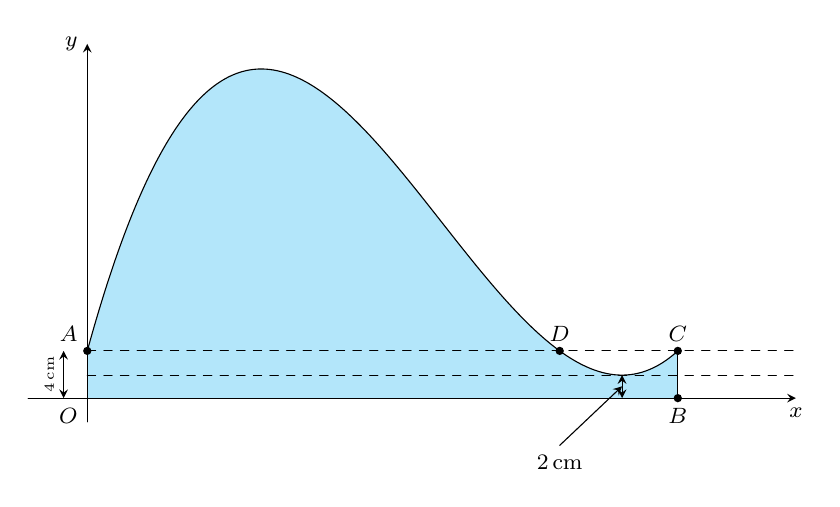
\begin{tikzpicture}[scale=0.15,font=\footnotesize,line join=round,line cap=round,declare function={f (\x)=(\x * (\x - 40) * (\x - 50)) / 550 + 4;},line join=round,line cap=round,>=stealth]
			\fill[cyan!30] (0,0) -- (50,0) -- (50,4) -- plot[domain=50:0,samples=100] ({\x},{f (\x)}) -- cycle;
			\draw[->] (-5,0) -- (60,0) node[below] {$x$};
			\draw[->] (0,-2) -- (0,30) node[left] {$y$};
			\node[below left] at (0,0) {$O$};
			\draw plot[smooth,domain=0:50,samples=150] ({\x},{f (\x)});
			\fill (0,4) circle (10pt) node[above left] {$A$};
			\fill (40,4) circle (10pt) node[above] {$D$};
			\fill (50,4) circle (10pt) node[above] {$C$};
			\fill (50,0) circle (10pt) node[below] {$B$};
			\draw[dashed] (0,4) -- (60,4);
			\draw (50,4) -- (50,0);
			\draw[dashed] (0,1.95) -- (60,1.95);
			\draw[<->] (45.28,0) -- (45.28,1.95);
			\draw[<-] (45.28,1)-- (40,-4) node[below] {$2$\,cm};
			\draw[<->] (-2,0) -- (-2,4) node[pos=0.5,sloped,above,font=\tiny] {$4$\,cm};
		\end{tikzpicture}
	}	
	\choiceTF
	{\True $d=4$}
	{\True $10b+c=2$}
	{Diện tích hình phẳng $(H)$ bằng $6\,674$\,cm$^2$ \textit{(tính theo đơn vị centimet vuông và làm tròn kết quả đến hàng đơn vị)}}
	{Khi cho $(H)$ quay quanh trục $Ox$ thì thể tích khối tròn xoay thu được bằng $4{,}3$\,m$^3$ \textit{(tính theo đơn vị mét khối và làm tròn kết quả đến hàng phần mười)}}
	\loigiai{
		\begin{itemchoice}
			\itemch Từ đồ thị, đường cong đi qua điểm $A(0;4)$ nên thay $x=0$ vào hàm số ta được $f(0)=4 \Rightarrow d=4$.
			\itemch Theo giả thiết $AD=40$\,cm, $BC=4$\,cm và $OB=50$\,cm nên đồ thị đi qua $A(0;4)$, $D(40;4)$, $C(50;4)$.\\
			Xét phương trình hoành độ giao điểm $f(x)-4=0$ có $3$ nghiệm $x=0$, $x=40$, $x=50$. Khi đó
			\allowdisplaybreaks
			\begin{eqnarray*}
				&&f(x)-4 = \dfrac{1}{550}x(x-40)(x-50)\\
				&\Leftrightarrow& f(x) - 4 = \dfrac{1}{550}(x^3-90x^2+2\,000x)\\
				&\Leftrightarrow& f(x) = \dfrac{1}{550}x^3 - \dfrac{9}{55}x^2 + \dfrac{40}{11}x + 4.
			\end{eqnarray*}
			Đồng nhất hệ số ta có $b = -\dfrac{9}{55}$ và $c = \dfrac{40}{11}$.\\
			Khi đó $10b+c = 10 \cdot \left(-\dfrac{9}{55}\right) + \dfrac{40}{11} = 2$.
			\itemch Diện tích hình phẳng $(H)$ là
			\[S = \displaystyle\int\limits_{0}^{50} \left( \dfrac{1}{550}x^3 - \dfrac{9}{55}x^2 + \dfrac{40}{11}x + 4 \right) \mathrm{\,d}x = \dfrac{8\,450}{11} \approx 768{,}18 \approx 768 \,(\text{cm}^2).\]
			\itemch Thể tích khối tròn xoay thu được là
			\[V = \pi \displaystyle\int\limits_{0}^{50} \big[f(x)\big]^2 \mathrm{\,d}x=\pi \displaystyle\int\limits_{0}^{50} \left(\dfrac{1}{550}x^3 - \dfrac{9}{55}x^2 + \dfrac{40}{11}x + 4\right)^2 \mathrm{\,d}x\approx 50\,793 \,(\text{cm}^3) \approx 0{,}05 \,(\text{m}^3).\]
		\end{itemchoice}
	}
\end{ex}
%%%=============================%%%

\caukq
%%%=============EX_17=============%%%
\begin{ex}%[2D1V3-6]%[TDMZZ15]%[Tên tác giả]
	Nhà máy X chuyên sản xuất một loại sản phẩm cho nhà máy Y. Hai nhà máy thỏa thuận rằng, hằng tháng nhà máy X cung cấp cho nhà máy Y số lượng sản phẩm theo đơn đặt hàng của nhà máy Y (tối đa $60$ tấn sản phẩm). Nếu số lượng đặt hàng là $x$ tấn sản phẩm thì giá bán cho mỗi tấn sản phẩm là $p(x)=65-0{,}02x^{2}$ (triệu đồng). Chi phí để nhà máy X sản xuất $x$ tấn sản phẩm trong một tháng là $C(x)=48+8{,}2x$ (triệu đồng), giả sử thuế mà nhà máy X phải đóng cho nhà nước là $10\%$ tổng doanh thu mỗi tháng. Hỏi mỗi tháng nhà máy X thu được lợi nhuận cao nhất là bao nhiêu triệu đồng (\textit{sau khi đã trừ thuế giá trị gia tăng, làm tròn kết quả đến hàng đơn vị}).
	\par
	\shortans[0]{975}
	\loigiai{
		Doanh thu mỗi tháng của nhà máy X khi bán $x$ tấn sản phẩm ($0 < x \le 60$) là
		\[R(x) = x \cdot p(x) = x\left(65 - 0{,}02x^2\right) = 65x - 0{,}02x^3 \text{ (triệu đồng)}.\]
		Sau khi đóng thuế $10\%$ doanh thu, doanh thu thực tế nhà máy giữ lại là $90\%$ doanh thu ban đầu.\\
		Lợi nhuận mỗi tháng (sau thuế) của nhà máy X là
		\begin{align*}
			L(x) &= 0{,}9 \cdot R(x) - C(x) \\
			&= 0{,}9\left(65x - 0{,}02x^3\right) - (48 + 8{,}2x) \\
			&= 58{,}5x - 0{,}018x^3 - 48 - 8{,}2x \\
			&= -0{,}018x^3 + 50{,}3x - 48 \text{ (triệu đồng)}.
		\end{align*}
		Xét hàm số $L(x) = -0{,}018x^3 + 50{,}3x - 48$ trên khoảng $(0; 60]$.\\
		Đạo hàm $L'(x) = -0{,}054x^2 + 50{,}3$.\\
		Ta có $L'(x) = 0 \Leftrightarrow x^2 = \dfrac{50{,}3}{0{,}054} = \dfrac{25\,150}{27} \Rightarrow x = \sqrt{\dfrac{25\,150}{27}} \approx 30{,}52$.\\
		Bảng biến thiên của hàm số $L(x)$ trên $(0; 60]$
		\begin{center}
			
\begin{tikzpicture}
				\tkzTabInit[nocadre=false, lgt=1.2, espcl=4, deltacl=0.5]
				{$x$/1.2, $L'(x)$/0.7, $L(x)$/2}
				{$0$, $\sqrt{\dfrac{25\,150}{27}}$, $60$}
				\tkzTabLine{,+,0,-,}
				\tkzTabVar{-/ $-48$, +/ $\approx 975$, -/ $-182{,}4$}
			\end{tikzpicture}
		\end{center}
		Dựa vào bảng biến thiên, ta thấy hàm số đạt giá trị lớn nhất tại $x = \sqrt{\dfrac{25\,150}{27}}$.\\
		Giá trị lợi nhuận lớn nhất tương ứng là
		\[\max\limits_{(0;60]} L(x) = L\left(\sqrt{\dfrac{25\,150}{27}}\right) \approx 975{,}44 \text{ (triệu đồng)}.\]
		Làm tròn kết quả đến hàng đơn vị, ta được $975$ triệu đồng.
	}
\end{ex}
%%%=============================%%%

%%%=============EX_18=============%%%
\begin{ex}%[1H8V6-2]
	Cho hình lăng trụ $ABC.A'B'C'$ có $AB=2$, $AC=3$, $\widehat{BAC}=60^{\circ}$ và chiều dài cạnh bên $AA'=3$. Biết hình chiếu vuông góc của $C$ trên đáy $(A'B'C')$ là trung điểm của cạnh $B'C'$. Hãy xác định số đo góc nhị diện $[C', A'B', A]$ theo đơn vị độ (\textit{làm tròn kết quả đến hàng đơn vị}).
	\par
	\shortans[0]{116}
	\loigiai{
		\begin{center}
			\begin{tikzpicture}[scale=1, font=\footnotesize, line join=round, line cap=round, >=stealth]
				\path
				(0,0) coordinate (A')
				(1.8,-1.5) coordinate (B')
				(4,0) coordinate (C')
				($(C')!1/2!(B')$) coordinate (H)
				($(H)+(0,4)$) coordinate (C)
				($(C)+(B')-(C')$) coordinate (B)
				($(C)+(A')-(C')$) coordinate (A)
				($(A')!0.3!(B')$) coordinate (E)
				($2*(B')-(H)$) coordinate (K)
				($(C')+(K)-(E)$) coordinate (I1)
				(intersection of A'--B' and K--I1) coordinate (I)
				(intersection of A'--B' and K--B) coordinate (x)
				(intersection of C'--B' and I--B) coordinate (y)
				;
				\draw (x)--(A')--(A)--(B)--(C)--(C')--(y)--(I)--(K)--cycle (A)--(C)--(H) (y)--(B)--(x);
				\draw[dashed] (A')--(C')--(E) (x)--(I) (K)--(y) (B)--(B');
				\foreach \p/\q in {A/180,B/90,C/0,A'/180,B'/180,C'/0,H/-80,E/-170,K/-200,I/0}
				\fill[black] (\p) circle (1.0pt) node[shift={(\q:3mm)}]{$\p$};
				\draw pic[draw=black, angle radius=0.2cm] {right angle = C--H--C'}
				pic[draw=black, angle radius=0.2cm] {right angle = B--K--B'}
				pic[draw=black, angle radius=0.2cm] {right angle = C'--E--A'}
				pic[draw=black, angle radius=0.2cm] {right angle = K--I--B'};
			\end{tikzpicture}
		\end{center}
		Gọi $H$ là trung điểm của $B'C'$.\\
		Theo giả thiết $CH \perp (A'B'C')$ nên chiều cao của lăng trụ là $h = CH$.\\
		Trong tam giác $A'B'C'$ có $A'B'=AB=2$, $A'C'=AC=3$ và $\widehat{B'A'C'} = \widehat{BAC} = 60^{\circ}$.\\
		Áp dụng định lý côsin trong tam giác $A'B'C'$, ta có
		\[B'C'^2 = A'B'^2 + A'C'^2 - 2A'B' \cdot A'C' \cdot \cos 60^{\circ} = 4 + 9 - 2 \cdot 2 \cdot 3 \cdot \dfrac{1}{2} = 7.\]
		Suy ra $B'C' = \sqrt{7}$ và $C'H = \dfrac{\sqrt{7}}{2}$.\\
		Gọi $K$ là hình chiếu vuông góc của $B$ trên $(A'B'C')$.\\
		Xét $\triangle CHC'$ vuông tại $H$ có $BK=CH = \sqrt{CC'^2 - C'H^2} = \sqrt{3^2 - \dfrac{7}{4}} = \dfrac{\sqrt{29}}{2}$.\\
		Kẻ $C'E \perp A'B'$ tại $E$, kẻ $KI \perp A'B'$ tại $I$.\\
		Ta có $\heva{& A'B'\perp BK \\ & A'B'\perp KI}\Rightarrow A'B'\perp BI$.\\
		Do đó số đo góc nhị diện $[C',A'B',A]$ là $180^{\circ}-\text{sđ}[K,A'B',A]=180^{\circ}-\widehat{BIK}$.\\
		Ta lại có $KI=\mathrm{d}(K,A'B')=\dfrac{1}{2}\mathrm{d}(C',A'B')=\dfrac{1}{2}C'E = \dfrac{1}{2}A'C' \cdot \sin 60^{\circ} = \dfrac{1}{2}\cdot 3 \cdot \dfrac{\sqrt{3}}{2} = \dfrac{3\sqrt{3}}{4}$.\\
		Trong $\triangle BKI$ vuông tại $K$, có $\tan\widehat{BIK}=\dfrac{BK}{KI}=\dfrac{\dfrac{\sqrt{29}}{2}}{\dfrac{3\sqrt{3}}{4}}=\dfrac{2\sqrt{57}}{9}\Rightarrow \widehat{BIK}\approx 64{,}24^{\circ}$.\\
		Vậy số đo góc nhị diện $[C',A'B',A]\approx 116^{\circ}$.
	}
\end{ex}
%%%=============================%%%

%%%=============EX_19=============%%%
\begin{ex}%[2D6C2-4]%[TDMZZ15-19-TLN]%[Nguyễn Văn Sang]
	Ban đầu cho hai hộp bi riêng biệt đựng những viên bi có cùng kích thước và cùng khối lượng. Hộp I đựng $x$ viên bi màu đỏ, $4$ viên bi màu xanh còn hộp II đựng $5$ viên bi màu đỏ và $3$ viên bi màu xanh. Tiến hành lấy ngẫu nhiên ba viên bi ở hộp I và hai viên bi ở hộp II, bỏ vào hộp III (ban đầu không có bi). Từ hộp III lấy ngẫu nhiên ra một viên bi. Biết rằng xác suất để viên bi lấy ra từ hộp III là của hộp I, nếu biết nó màu đỏ, không nhỏ hơn $0{,}6$. Hãy xác định giá trị nhỏ nhất của $x$.
	\begin{center}
		\begin{tikzpicture}[scale=0.85, font=\footnotesize, line join=round, line cap=round, >=stealth]
			% --- Vẽ Hộp I ---
			\draw[thick, blue!60!black, rounded corners=4pt] (0,2) rectangle (3,4.2);
			\node[above, blue!60!black] at (1.5,4.2) {\textbf{Hộp I}};
			% Bi đỏ hộp I (x bi)
			\shade[ball color=red] (0.6,2.5) circle (0.2);
			\shade[ball color=red] (1.1,2.5) circle (0.2);
			\node[red!80!black] at (1.65,2.5) {$\dots$};
			\shade[ball color=red] (2.4,2.5) circle (0.2);
			% Bi xanh hộp I (4 bi)
			\foreach \i in {1,2,3,4} \shade[ball color=blue] (0.3+0.6*\i, 3.3) circle (0.2);
			\node[below] at (1.5,2) {\textit{$x$ bi Đỏ, $4$ bi Xanh}};
			% --- Vẽ Hộp II ---
			\draw[thick, red!60!black, rounded corners=4pt] (6,2) rectangle (9,4.2);
			\node[above, red!60!black] at (7.5,4.2) {\textbf{Hộp II}};
			% Bi đỏ hộp II (5 bi)
			\foreach \i in {1,2,3,4,5} \shade[ball color=red] (6.15+0.45*\i, 2.5) circle (0.2);
			% Bi xanh hộp II (3 bi)
			\foreach \i in {1,2,3} \shade[ball color=blue] (6.3+0.6*\i, 3.3) circle (0.2);
			\node[below] at (7.5,2) {\textit{$5$ bi Đỏ, $3$ bi Xanh}};
			% --- Vẽ Hộp III ---
			\draw[very thick, orange!80!black, fill=orange!5, rounded corners=4pt] (3,-1.8) rectangle (6,0.2);
			\node[below, orange!80!black] at (4.5,-1.8) {\textbf{Hộp III (Rổ III)}};
			\node at (4.5,-0.8) {\scriptsize (Tổng 5 bi)};
			% --- Mũi tên cong chuyển bi (tránh đè chữ) ---
			\draw[->, line width=1.5pt, blue!60, opacity=0.9] (1.5,1.5) to[out=-70, in=160] (3,-0.2);
			\node[blue!80!black, left] at (1.9, 0.8) {\textbf{Lấy 3 bi}};
			\draw[->, line width=1.5pt, red!60, opacity=0.9] (7.5,1.5) to[out=-110, in=20] (6,-0.2);
			\node[red!80!black, right] at (7.1, 0.8) {\textbf{Lấy 2 bi}};
			% --- Kết quả cuối cùng ---
			\draw[->, thick, green!60!black] (4.5,-2.4) -- (4.5,-3.4);
			\node[below] at (4.5,-3.4) {Lấy ngẫu nhiên \textbf{1 bi Đỏ}};
		\end{tikzpicture}
	\end{center}
	\par
	\shortans[0]{7}
	\loigiai{
		Hộp III chứa $3$ bi từ hộp I và $2$ bi từ hộp II (tổng cộng $5$ bi). Gọi $H_1$ là biến cố viên bi lấy từ hộp III có nguồn gốc từ hộp I, $H_2$ là biến cố viên bi có nguồn gốc từ hộp II. Ta có
		\[\mathrm{P}(H_1) = \dfrac{3}{5}; \quad \mathrm{P}(H_2) = \dfrac{2}{5}.\]
		Gọi $A$ là biến cố lấy được viên bi màu đỏ. Tỷ lệ bi đỏ trong hộp I là $\dfrac{x}{x+4}$ và trong hộp II là $\dfrac{5}{8}$. Do đó, xác suất lấy được bi đỏ tương ứng với mỗi nguồn gốc là
		\[\mathrm{P}(A \mid H_1) = \dfrac{x}{x+4}; \quad \mathrm{P}(A \mid H_2) = \dfrac{5}{8}.\]
		\textbf{Sơ đồ hình cây xác suất:}
		\begin{center}
			\begin{tikzpicture}[
				level 1/.style={sibling distance=6cm, level distance=2.2cm},
				level 2/.style={sibling distance=3cm, level distance=2.5cm},
				edge from parent/.style={draw, thick, -stealth},
				every node/.style={font=\small, align=center}
				]
				\node {\textbf{Lấy 1 bi từ Hộp III}}
				child { node[draw, rounded corners, inner sep=4pt] {$H_1$ (Bi thuộc Hộp I)}
					child { node {\textbf{\color{red}Đỏ ($A$)}}
						edge from parent node[left, color=red!70!black, xshift=-1mm] {$\frac{x}{x+4}$}
					}
					child { node {\textbf{\color{blue}Xanh ($\overline{A}$)}}
						edge from parent node[right, color=blue!70!black, xshift=1mm] {$\frac{4}{x+4}$}
					}
					edge from parent node[above left, blue!80!black, xshift=-1mm] {$\mathrm{P}(H_1) = \frac{3}{5}$}
				}
				child { node[draw, rounded corners, inner sep=4pt] {$H_2$ (Bi thuộc Hộp II)}
					child { node {\textbf{\color{red}Đỏ ($A$)}}
						edge from parent node[left, color=red!70!black, xshift=-1mm] {$\frac{5}{8}$}
					}
					child { node {\textbf{\color{blue}Xanh ($\overline{A}$)}}
						edge from parent node[right, color=blue!70!black, xshift=1mm] {$\frac{3}{8}$}
					}
					edge from parent node[above right, blue!80!black, xshift=1mm] {$\mathrm{P}(H_2) = \frac{2}{5}$}
				};
			\end{tikzpicture}
		\end{center}
		Xác suất để lấy được bi đỏ là
		\[\mathrm{P}(A) = \mathrm{P}(H_1)\mathrm{P}(A \mid H_1) + \mathrm{P}(H_2)\mathrm{P}(A \mid H_2) = \dfrac{3}{5} \cdot \dfrac{x}{x+4} + \dfrac{2}{5} \cdot \dfrac{5}{8} = \dfrac{3x}{5(x+4)} + \dfrac{1}{4}.\]
		Xác suất để viên bi đó thuộc hộp I khi biết nó màu đỏ (áp dụng công thức Bayes) là
		\[\mathrm{P}(H_1 \mid A) = \dfrac{\mathrm{P}(H_1 \cap A)}{\mathrm{P}(A)} = \dfrac{\dfrac{3x}{5(x+4)}}{\dfrac{3x}{5(x+4)} + \dfrac{1}{4}} = \dfrac{12x}{17x + 20}.\]
		Theo giả thiết bài toán, xác suất này không nhỏ hơn $0{,}6$, nên ta có
		\[\mathrm{P}(H_1 \mid A) \ge 0{,}6 \Leftrightarrow \dfrac{12x}{17x+20} \ge \dfrac{3}{5} \Leftrightarrow 60x \ge 51x + 60 \Leftrightarrow 9x \ge 60 \Leftrightarrow x \ge \dfrac{20}{3} \approx 6{,}67.\]
		Vì $x$ là số viên bi ($x \in \mathbb{N}^*$) nên giá trị nhỏ nhất của $x$ thỏa mãn là $x = 7$.
	}
\end{ex}
%%%=============================%%%

%%%=============EX_20=============%%%
\begin{ex}%[2D4C3-2]%[TDMZZ15]%[Trương Tường]
	\immini[thm]{
		Trên một mảnh đất hình vuông $ABCD$ có cạnh bằng $60$ mét, đường parabol $(P_1)$ có trục đối xứng vuông góc với cạnh $CD$, đi qua hai điểm $D$, $E$, có đỉnh cách cạnh $CD$ một khoảng là $12$ mét. Gọi $(P_2)$ là đường parabol đối xứng với $(P_1)$ qua đường thẳng $GK$, $(H)$ là hình phẳng giới hạn bởi $(P_2)$ và các cạnh $AB$, $BC$ được tô màu như hình vẽ. Hãy tính diện tích phần tô màu theo đơn vị mét vuông (\textit{không làm tròn các phép tính trung gian và kết quả cuối cùng được làm tròn đến hàng phần trăm}).
	}{
		\begin{tikzpicture}[scale=.75, >=stealth, line join=round, line cap=round, font=\footnotesize]
			\def\a{6}
			\path (0,0) coordinate (A)
			++(0:\a) coordinate (B)
			++(90:\a) coordinate (C)
			++($(A)-(B)$) coordinate (D)
			($(D)!.3!(C)$) coordinate (E)
			($(D)!.5!(E)$)++(-90:\a/5) coordinate (O)
			($(C)!1/6!(B)$) coordinate (K)
			($(A)!1/6!(B)$) coordinate (G)
			($2*(G)!(D)!(K)-(D)$) coordinate (D')
			($2*(G)!(E)!(K)-(E)$) coordinate (E')
			($2*(G)!(O)!(K)-(O)$) coordinate (O')
			;
			\begin{scope}
				\clip (A)--(B)--(C)--(D)--cycle;
				\draw [fill=cyan, rotate around={-90:(O')}] (E') parabola bend (O') (D');
			\end{scope}
			\draw [dash pattern=on 1.5pt off 1.5pt] (K)--++(180:.35) (G)--++(90:.35);
			\draw [<->] (C)++(180:.35)--++($(K)-(C)$) node [above, sloped, pos=.5] {$10\,\text{m}$};
			\draw [<->] (A)++(90:.35)--++($(G)-(A)$) node [above, sloped, pos=.5] {$10\,\text{m}$};
			\path (D)--(E) node [above, sloped, pos=.5] {$18\,\text{m}$}
			(O) node [below] {$(P_1)$}
			(B)++(135:.6) node[rotate=45] {$(P_2)$};
			\draw (A)--(B)--(C)--(D)--cycle node [above, sloped, pos=.5] {$60\,\text{m}$}
			(G)--(K)
			(D) parabola bend (O) (E);
			\foreach \x/\y in {A/-135, B/-45, C/45, D/135, E/45, G/-90, K/0}{
				\draw [fill=black] (\x) circle (1pt) ++(\y:0.4) node {$\x$};
			}
		\end{tikzpicture}
	}
	\par
	\shortans[0]{2,95}
	\loigiai{
		\begin{center}
			\begin{tikzpicture}[scale=1, >=stealth, line join=round, line cap=round, font=\footnotesize]
				\def\a{6}
				\path (0,0) coordinate (A)
				++(0:\a) coordinate (B)
				++(90:\a) coordinate (C)
				++($(A)-(B)$) coordinate (D)
				($(D)!.3!(C)$) coordinate (E)
				($(D)!.5!(E)$)++(-90:\a/5) coordinate (O)
				($(C)!1/6!(B)$) coordinate (K)
				($(A)!1/6!(B)$) coordinate (G)
				($2*(G)!(D)!(K)-(D)$) coordinate (D')
				($2*(G)!(E)!(K)-(E)$) coordinate (E')
				($2*(G)!(O)!(K)-(O)$) coordinate (O')
				(K)+($(G)-(B)$) coordinate (I)
				;
				\begin{scope}
					\clip (G)--(B)--(K)--(I)--cycle;
					\draw [fill=cyan] (D) parabola bend (O) (E);
					\draw [fill=cyan, rotate around={-90:(O')}] (E') parabola bend (O') (D');
				\end{scope}
				\path (D)--(E) node [above, sloped, pos=.5] {$18\,\text{m}$}
				(A)--(G)
				(C)--(K)
				(E)++(-90:.4) node [right] {$(P_1)$}
				(B)++(135:.6) node [rotate=45] {$(P_2)$}
				;
				\draw (A)--(B)--(C)--(D)--cycle node [above, sloped, pos=.5] {$60\,\text{m}$}
				(G)--(K)
				(D) parabola bend (O) (E)
				(G)--(I)--(K)
				(D)--($(D)!(O)!(E)$) node [below, pos=.5] {$9\,\text{m}$}
				;
				\draw [dash pattern=on 1.5pt off 1.5pt] (D)--++(180:.6) (O)--++(180:1.5) (O)--++(0:1) (O)--($(D)!(O)!(E)$);
				\draw [<->] (C)++(180:.35)--++($(K)-(C)$) node [above, sloped, pos=.5] {$10\,\text{m}$};
				\draw [<->] (A)++(90:.35)--++($(G)-(A)$) node [above, sloped, pos=.5] {$10\,\text{m}$};
				\draw [<->] (O)++(180:1.5)--++($(D)!.5!(E)-(O)$) node [below, pos=.5, sloped] {$12\,\text{m}$};
				\draw [<->] (O)++(0:1)--++(90:.2) node [right, pos=.5] {$2\,\text{m}$};
				\foreach \x/\y in {A/-135, B/-45, C/45, D/90, E/90, O/-110, G/-90, K/0, I/135}{
					\draw [fill=black] (\x) circle (1pt) ++(\y:0.3) node {$\x$};
				}
			\end{tikzpicture}
			\hspace*{.25cm}
			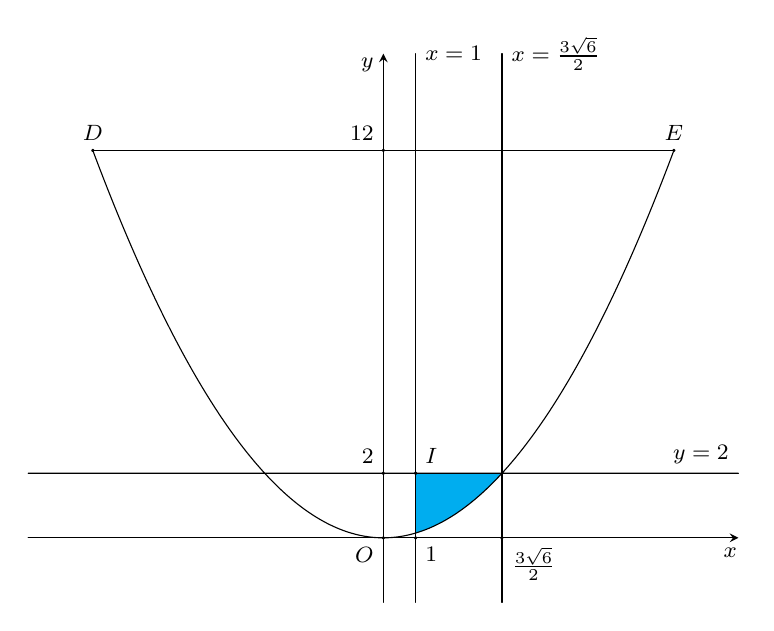
\begin{tikzpicture}[scale=.41, >=stealth, line join=round, line cap=round, font=\footnotesize]
				\def\xmin{-11} \def\xmax{11} \def\ymin{-2} \def\ymax{15}
				\tikzset{declare function={f(\x)=4/27*(\x)^2;x0=3*sqrt(6)/2;}}
				\fill [smooth, samples=100, cyan] plot [domain=1:x0] ({\x},{f(\x)})--(1,2)--cycle;
				\draw [smooth, samples=100] plot [domain=-9:9] ({\x},{f(\x)})
				plot [domain=\xmin:\xmax] ({\x},{2}) node [above left] {$y=2$}
				;
				\draw (1,\ymin)--(1,\ymax) node [right] {$x=1$}
				(x0,\ymin)--(x0,\ymax) node [right] {$x=\frac{3\sqrt{6}}{2}$}
				(-9,12)--(9,12)
				;
				\draw [->] (\xmin,0)--(\xmax,0) node [below, xshift=-3pt] {$x$};
				\draw [->] (0,\ymin)--(0,\ymax) node [left, yshift=-4pt] {$y$};
				\draw [fill=black] (0,0) circle (1pt) node [below left] {$O$}
				(1,2) circle (1pt) node [above right] {$I$}
				(0,2) circle (1pt) node [above left] {$2$}
				(0,12) circle (1pt) node [above left] {$12$}
				(1,0) circle (1pt) node [below right] {$1$}
				(x0,0) circle (1pt) node [below right] {$\frac{3\sqrt{6}}{2}$}
				(-9,12) circle (1pt) node [above] {$D$}
				(9,12) circle (1pt) node [above] {$E$}
				;
			\end{tikzpicture}
		\end{center}
		Gọi $I$ là đỉnh thứ tư của hình vuông $BKIG$.\\
		Gọi $(H')$ là phần hình phẳng giới hạn bởi $(P_1)$ và hai cạnh $IG$, $IK$.\\
		Khi đó $(H)$ và $(H')$ đối xứng qua đường thẳng $GK$ nên chúng có diện tích bằng nhau.\\
		Chọn hệ trục tọa độ $Oxy$ sao cho gốc tọa độ $O$ trùng với đỉnh của $(P_1)$, trục $Oy$ trùng với trục đối xứng của $(P_1)$ như hình trên (đơn vị trên mỗi trục là mét).\\
		Ta có $E(9;12)$, $I(1;2)$.\\
		Phương trình $(P_1)$ có dạng $y=f(x)=ax^2$.\\
		Vì $(P_1)$ đi qua $E$ nên ta có $a \cdot 9^2=12 \Leftrightarrow a=\dfrac{4}{27}$.\\
		Suy ra phương trình của $(P_1)$ là $y=\dfrac{4}{27}x^2$.\\
		Đường thẳng $IK$ có phương trình $y=2$.\\
		Xét phương trình hoành độ giao điểm
		\[\dfrac{4}{27}x^2=2 \Leftrightarrow x^2=\dfrac{27}{2} \Leftrightarrow x=\pm \dfrac{3\sqrt{6}}{2}.\]
		Do đó, đoạn thẳng $IK$ cắt $(P_1)$ tại điểm có hoành độ $x = \dfrac{3\sqrt{6}}{2}$.\\
		Phần hình phẳng $(H')$ được giới hạn bởi hai đồ thị $y=\dfrac{4}{27}x^2$, $y=2$ và hai đường thẳng $x=1$, $x=\dfrac{3\sqrt{6}}{2}$ nên có diện tích là
		\[S=\displaystyle\int\limits_1^{\frac{3\sqrt{6}}{2}} \left(2-\dfrac{4}{27}x^2\right) \mathrm{\,d}x \approx 2{,}95 \text{ (m}^2\text{)}.\]
		Vậy diện tích phần tô màu xấp xỉ $2{,}95$ m$^2$.
	}
\end{ex}
%%%=============================%%%

%%%=============EX_21=============%%%
\begin{ex}%[2H5C3-4]%[TDMZZ13]%[Nguyễn Đức Tuấn Anh]
	Trong không gian $Oxyz$ có đơn vị dài trên mỗi trục là mét, có hai vật X và Y chuyển động trên hai đường tròn. Biết vật X ở ba thời điểm khác nhau có ba vị trí là $A(-2;-3;0)$, $B(1;-4;0)$, $C\left(0;1+2\sqrt{6};0\right)$, vật Y ở ba thời điểm khác nhau có ba vị trí là $E(1;0;2)$, $F(-1;2;2)$, $G(1;4;2)$. Hãy xác định khoảng cách ngắn nhất có thể giữa hai vật X và Y theo đơn vị centimet (\textit{không làm tròn các phép tính trung gian và làm tròn kết quả cuối cùng đến hàng đơn vị}).
	\par
	\shortans[0]{283}
	\loigiai{
		\begin{center}
			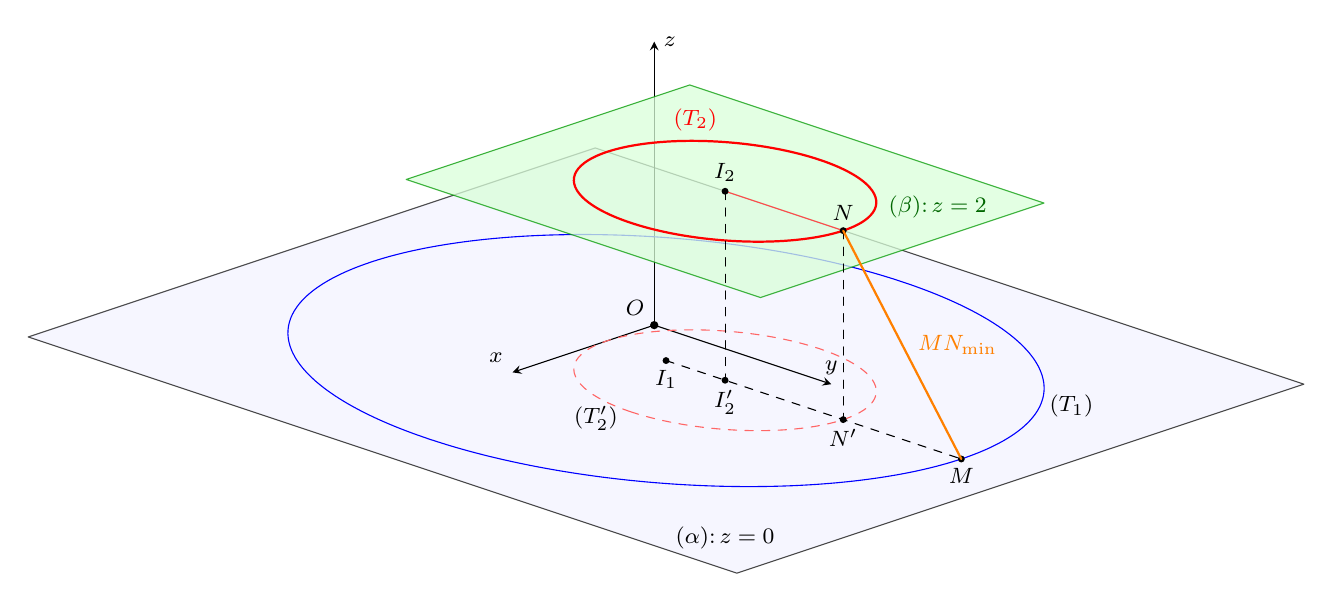
\begin{tikzpicture}[x={(-0.6cm, -0.2cm)}, y={(0.75cm, -0.25cm)}, z={(0cm, 1.2cm)}, font=\footnotesize, line join=round, line cap=round, >=stealth]
				% ==========================================
				\draw[fill=blue!5, opacity=0.7]
				(-5,-5,0) -- (7,-5,0) -- (7,7,0) -- (-5,7,0) -- cycle;
				\node[] at (6,6,0) {$(\alpha)\colon z=0$};
				\draw[->] (0,0,0) -- (3,0,0) node[above left] {$x$};
				\draw[->] (0,0,0) -- (0,3,0) node[above] {$y$};
				\draw[->] (0,0,0) -- (0,0,3) node[right] {$z$};
				\fill (0,0,0) circle (1.5pt) node[above left] {$O$};
				% (T1)
				\draw[blue, smooth] plot[domain=0:360, samples=100, variable=\t] ({1+5*cos(\t)}, {1+5*sin(\t)}, 0);
				\node at ({1+5*cos(120)}, {1+5*sin(120)}, 0) [right] {$(T_1)$};
				% (T'2)
				\draw[red!60, dashed, smooth] plot[domain=0:360, samples=100, variable=\t] ({1+2*cos(\t)}, {2+2*sin(\t)}, 0);
				\node at ({1+2*cos(-20)}, {2+2*sin(-20)}, 0)[below] {$(T'_2)$};
				% Các điểm và đường nối tâm trên mặt phẳng alpha
				\draw[dashed] (1,1,0) -- (1,6,0);
				\fill (1,1,0) circle (1.25pt) node[below] {$I_1$};
				\fill (1,2,0) circle (1.25pt) node[below] {$I'_2$};
				\fill (1,4,0) circle (1.25pt) node[below] {$N'$};
				\fill (1,6,0) circle (1.25pt) node[below] {$M$};
				% ==========================================
				\draw[draw=green!60!black, fill=green!15, opacity=0.75]
				(-2,-1,2) -- (4,-1,2) -- (4,5,2) -- (-2,5,2) -- cycle;
				\node[green!40!black] at (1.5,6,2.75) {$(\beta)\colon z=2$};
				% Đường tròn (T2)
				\draw[thick, red, smooth] plot[domain=0:360, samples=100, variable=\t] ({1+2*cos(\t)}, {2+2*sin(\t)}, 2);
				\node[red] at ({1+2*cos(230)}, {2+2*sin(230)}, 2) [above] {$(T_2)$};
				% Các điểm trên mặt phẳng beta
				\draw[red!70] (1,2,2) -- (1,4,2);
				\fill (1,2,2) circle (1.25pt) node[above] {$I_2$};
				\fill (1,4,2) circle (1.25pt) node[above] {$N$};
				% ==========================================
				\draw[dashed] (1,2,2) -- (1,2,0) (1,4,2) -- (1,4,0);
				\draw[thick, orange] (1,6,0) -- (1,4,2) node[midway, right, xshift=2pt] {$MN_{\min}$};
			\end{tikzpicture}
		\end{center}
		Các điểm $A$, $B$, $C$ đều có cao độ $z=0$ nên thuộc mặt phẳng $(\alpha) \colon z=0$.\\
		Do đó quỹ đạo của vật X là đường tròn $(T_1)$ nằm trong mặt phẳng $(\alpha)$.\\
		Tương tự các điểm $E$, $F$, $G$ đều có cao độ $z=2$ nên thuộc mặt phẳng $(\beta) \colon z=2$.\\
		Do đó quỹ đạo của vật Y là đường tròn $(T_2)$ nằm trong mặt phẳng $(\beta)$.\\
		Mặt phẳng $(\alpha)$ song song với mặt phẳng $(\beta)$ và khoảng cách giữa chúng bằng $\mathrm{d}\big((\alpha), (\beta)\big) = 2$.\\
		Phương trình đường tròn $(T_1)$ trong mặt phẳng $(\alpha)$ có dạng $x^2+y^2-2ax-2by+c=0$.\\
		Thay tọa độ $A$, $B$, $C$ vào ta có hệ phương trình
		\[
		\heva{& 4+9+4a+6b+c=0 \\ & 1+16-2a+8b+c=0 \\ & 0+\left(1+2\sqrt{6}\right)^2-0-2\left(1+2\sqrt{6}\right)b+c=0} \Leftrightarrow \heva{& a=1 \\ & b=1 \\ & c=-23.}
		\]
		Suy ra đường tròn $(T_1)$ có tâm $I_1(1;1;0)$ và bán kính $R_1 = \sqrt{1^2+1^2-(-23)} = 5$.\\
		Phương trình đường tròn $(T_2)$ trong mặt phẳng $(\beta)$ có dạng $x^2+y^2-2px-2qy+r=0$.\\
		Thay tọa độ của $E$, $F$, $G$ vào ta có hệ phương trình
		\[
		\heva{& 1+0-2p+r=0 \\ & 1+4+2p-4q+r=0 \\ & 1+16-2p-8q+r=0} \Leftrightarrow \heva{& p=1 \\ & q=2 \\ & r=1.}
		\]
		Suy ra đường tròn $(T_2)$ có tâm $I_2(1;2;2)$ và bán kính $R_2 = \sqrt{1^2+2^2-1} = 2$.\\
		Gọi $(T'_2)$ là hình chiếu vuông góc của $(T_2)$ lên mặt phẳng $(\alpha)$. Khi đó $(T'_2)$ là đường tròn có tâm $I'_2(1;2;0)$ và bán kính $R'_2 = R_2 = 2$.\\
		Gọi $M$ và $N$ lần lượt là vị trí của vật X và vật Y. Gọi $N'$ là hình chiếu vuông góc của $N$ lên $(\alpha)$.\\
		Khi đó $M \in (T_1)$, $N \in (T_2)$ và $N' \in (T'_2)$.\\
		Khoảng cách $MN = \sqrt{NN'^2 + MN'^2} = \sqrt{2^2 + MN'^2}$.\\
		Do độ dài $NN' = \mathrm{d}\big((\alpha), (\beta)\big) = 2$ không đổi nên $MN$ đạt giá trị nhỏ nhất khi và chỉ khi $MN'$ đạt giá trị nhỏ nhất.\\
		Ta có
		\[I_1I'_2 = \sqrt{(1-1)^2 + (2-1)^2 + 0} = 1.\]
		Do $I_1I'_2 = 1 < R_1 - R'_2 = 5 - 2 = 3$ nên đường tròn $(T'_2)$ nằm hoàn toàn bên trong đường tròn $(T_1)$.\\
		Khoảng cách ngắn nhất giữa hai điểm lần lượt nằm trên hai đường tròn này bằng
		\[MN'_{\min} = R_1 - R'_2 - I_1I'_2 = 5 - 2 - 1 = 2.\]
		Suy ra $MN_{\min} = \sqrt{2^2 + 2^2} = 2\sqrt{2} \text{ (m)} \approx 283 \text{ (cm)}$.
	}
\end{ex}
%%%=============================%%%

%%%=============EX_22=============%%%
\begin{ex}%[2D6C1-2]
	Xếp ngẫu nhiên hai học sinh lớp A, hai học sinh lớp B, hai học sinh lớp C vào $3$ phòng học. Hãy tính xác suất để sao cho không có hai học sinh cùng lớp cùng phòng, nếu đã biết mỗi phòng có ít nhất một học sinh (\textit{không làm tròn ở các phép tính trung gian và làm tròn kết quả cuối cùng đến hàng phần trăm}).
	\par
	\shortans[0]{0,36}
	\loigiai{
		Gọi $A$ là biến cố \lq\lq không có hai học sinh cùng lớp cùng phòng\rq\rq.\\
		Gọi $B$ là biến cố \lq\lq mỗi phòng có ít nhất một học sinh\rq\rq.\\
		Ta có $\mathrm{P}(A \mid B)=\dfrac{n(AB)}{n(B)}=\dfrac{n(A)-n\left(A\overline{B}\right)}{n(B)}$.
		\begin{itemize}
			\item Tính $n(A)$:
			\begin{itemize}
				\item Xếp $2$ học sinh lớp A để không có $2$ học sinh lớp A cùng phòng, có $\mathrm{A}_3^2=6$ cách xếp.
				\item Xếp $2$ học sinh lớp B để không có $2$ học sinh lớp B cùng phòng, có $\mathrm{A}_3^2=6$ cách xếp.
				\item Xếp $2$ học sinh lớp C để không có $2$ học sinh lớp C cùng phòng, có $\mathrm{A}_3^2=6$ cách xếp.
			\end{itemize}
			Do đó $n(A)=6^3=216$.
			\item Tính $n(B)$, có các khả năng sau:
			\begin{itemize}
				\item Hai phòng mỗi phòng có $1$ học sinh, một phòng có $4$ học sinh. Có $\mathrm{C}_3^1 \cdot \mathrm{C}_6^1 \cdot \mathrm{C}_5^1 \cdot \mathrm{C}_4^4=90$ (cách xếp).
				\item Một phòng có $1$ học sinh, một phòng có $2$ học sinh, một phòng có $3$ học sinh. Có $3! \cdot \mathrm{C}_6^1 \cdot \mathrm{C}_5^2 \cdot \mathrm{C}_3^3=360$ (cách xếp).
				\item Mỗi phòng có $2$ học sinh. Có $\mathrm{C}_6^2 \cdot \mathrm{C}_4^2 \cdot \mathrm{C}_2^2=90$ (cách xếp).
			\end{itemize}
			Do đó $n(B)=90+360+90=540$.
			\item Tính $n\left(A\overline{B}\right)$:\\
			Ta có $\overline{B}$ là biến cố \lq\lq có phòng không có học sinh nào\rq\rq.\\
			Tức là khi $\overline{B}$ xảy ra thì có trường hợp có $1$ phòng trống, hoặc trường hợp có $2$ phòng trống.\\
			Suy ra $A\overline{B}$ là biến cố \lq\lq không có hai học sinh cùng lớp cùng phòng và có $1$ phòng trống\rq\rq.\\
			Do đó $n\left(A\overline{B}\right)=\mathrm{C}_3^1 \cdot 2! \cdot 2! \cdot 2!=24$.
		\end{itemize}
		Vậy $\mathrm{P}(A \mid B)=\dfrac{n(AB)}{n(B)}=\dfrac{n(A)-n\left(A\overline{B}\right)}{n(B)}=\dfrac{216-24}{540}\approx 0{,}36$.
	}
\end{ex}